\documentclass[11pt,a4paper]{article}

\usepackage[margin=2.5cm]{geometry}
\usepackage[T1]{fontenc}
\usepackage{lmodern}
\usepackage{microtype}
\usepackage{parskip}
\usepackage{setspace}
\usepackage{graphicx}
\usepackage{xcolor}
\usepackage[hidelinks]{hyperref}
\usepackage{fancyhdr}
\usepackage{booktabs}
\usepackage{listings}
\usepackage{tikz}

\usetikzlibrary{positioning, arrows.meta, calc, fit, backgrounds}

\setstretch{1.15}

\lstset{
  basicstyle=\ttfamily\small,
  frame=single,
  rulecolor=\color{black!30},
  backgroundcolor=\color{black!3},
  columns=fullflexible,
  breaklines=true,
  showstringspaces=false,
  xleftmargin=0.5em,
  xrightmargin=0.5em
}

\graphicspath{{figures/}}

\definecolor{icdecred}{HTML}{A51C24}

\setlength{\headheight}{25pt}
\pagestyle{fancy}
\fancyhf{}
\fancyhead[L]{
\includegraphics[height=0.6cm]{icdec-logo}}
\fancyhead[R]{\small ICDeCompiler v1.0}
\fancyfoot[C]{\thepage}

\newcommand{\version}{1.0}

\begin{document}

\begin{titlepage}
  \noindent
  
\includegraphics[height=2cm]{pme-logo}\hfill
\includegraphics[height=2cm]{icdec-logo}

  \vspace*{3.5cm}
  {\color{icdecred}\rule{\linewidth}{2pt}}

  \vspace{1.2cm}
  \begin{center}
    {\fontsize{44}{52}\selectfont\bfseries ICDeCompiler}\\[0.8em]
    {\LARGE Technical Documentation}
  \end{center}

  \vspace{1.2cm}
  {\color{icdecred}\rule{\linewidth}{2pt}}

  \vfill
  \begin{center}
    \begin{tabular}{ll}
      Version    & \version \\
      Date       & \today \\
      Status     & Pending \\
      Repository & \texttt{github.com/beepbeepbeepp/icdecompiler}
    \end{tabular}
  \end{center}

  \vspace{1.5cm}
  \begin{center}
    {\large Muhammad Faudzan Abdullah}\\[0.3em]
    Pusat Mikroelektronika ITB \& ICDeC
  \end{center}
\end{titlepage}

\tableofcontents
\newpage

\section{Background}

The lab is developing its own RISC-V system-on-chip together with a custom
accelerator for neural network inference. To be useful, that hardware needs a
way to run trained models on it.

For commercial platforms this path already exists. Arm's Ethos-U, for example,
comes with Vela, which compiles a quantized model for the accelerator, and a
runtime that executes it. These tools are tied to their own hardware and
cannot target a custom design. General-purpose ML compilers are a closer fit
in principle, but their import paths for quantized models are not stable
enough to build on, and they assume toolchains the lab's targets do not use.

Without a compiler, every model has to be ported by hand: each layer rewritten
in C, the quantization arithmetic reproduced exactly, and the split between CPU
and accelerator decided manually. This is slow, has to be repeated for every
model and every change to a model, and errors in the arithmetic are easy to
make and hard to see.

The targets add one more constraint. The RISC-V cores in this SoC use a GCC
toolchain with extensions such as hardware loops and SIMD instructions that
LLVM does not support. A compiler that ends in LLVM IR would lose them.
ICDeCompiler therefore stops at C and leaves final code generation to the
target's own GCC.

ICDeCompiler was built to close this gap: a compiler for the lab's own SoC and
accelerator, from trained model to code that runs on the hardware. It is built
on MLIR, part of the LLVM project.

\section{Goals}

ICDeCompiler is designed around a few simple goals.

\begin{enumerate}
  \item \textbf{From model to code in one step.} A trained model goes in, and
    C code ready to be added to the firmware comes out. No layer has to be
    rewritten by hand.

  \item \textbf{The accelerator is optional.} The same model can run on the
    CPU alone or with its heavy computation sent to the accelerator. Both give
    the same results.

  \item \textbf{Checked before it reaches the board.} The generated code can
    be tested on a PC against the original model. Mistakes are found early,
    where they are easy to fix.

  \item \textbf{Made for small devices.} The generated code needs no operating
    system, no dynamic memory and no extra libraries, so it fits on bare-metal
    microcontrollers.

  \item \textbf{Easy to start with.} A ready-made release includes everything
    needed to use the compiler, so there is no need to build it from source
    first.

  \item \textbf{Hardware can change without breaking the compiler.} The
    compiler talks to the accelerator only through a small driver interface.
    If the hardware changes, only the driver needs to be updated.
\end{enumerate}

\subsection*{What ICDeCompiler does not do}

ICDeCompiler does not train or quantize models; that is done beforehand with
the usual tools. It works with inputs of fixed size only. It also does not yet
try to make the generated code fast: the first priority is that the results are
correct.

\section{Overview}

ICDeCompiler turns a trained model into C code in three stages. The model is
first prepared by \texttt{model-tools}, which separates the weights from the
structure of the network. The structure is then compiled into C by the
compiler itself. Finally, the generated code is built into the firmware with
the target's own toolchain.

\begin{figure}[h]
\centering
\begin{tikzpicture}[
    node distance=0.8cm and 1.0cm,
    box/.style={draw, rounded corners=3pt, align=center,
                minimum width=3.6cm, minimum height=1.05cm, font=\small},
    file/.style={box, fill=black!4},
    tool/.style={box, fill=icdecred!8, draw=icdecred},
    hw/.style={box, fill=black!12},
    arrow/.style={-{Stealth[length=2.2mm]}, thick}
  ]

  \node[file] (model) {Trained model\\[-1pt]\footnotesize .tflite or SavedModel};
  \node[tool, below=of model] (mt) {model-tools\\[-1pt]\footnotesize separate weights and structure};
  \node[file, below left=of mt] (w) {Weights\\[-1pt]\footnotesize \texttt{net\_weights.c/.h}};
  \node[file, below right=of mt] (mlir) {Model structure\\[-1pt]\footnotesize \texttt{net.mlir}};
  \node[tool, below=of mlir] (cc) {ICDeCompiler\\[-1pt]\footnotesize split CPU and accelerator};
  \node[file, below=of cc] (c) {Inference code\\[-1pt]\footnotesize \texttt{net.c}};
  \node[file] (fw) at ($(w |- c)!0.5!(c) + (0,-1.9)$) {Firmware\\[-1pt]\footnotesize \texttt{main.c}, drivers};
  \node[box, below=of fw] (gcc) {Target GCC};
  \node[hw, below=1.8cm of gcc] (soc) {RISC-V SoC\\[-1pt]\footnotesize CPU and accelerator};

  \draw[arrow] (model) -- (mt);
  \draw[arrow] (mt.west) -| (w.north);
  \draw[arrow] (mt.east) -| (mlir.north);
  \draw[arrow] (mlir) -- (cc);
  \draw[arrow] (cc) -- (c);
  \draw[arrow] (w.south) |- (fw.west);
  \draw[arrow] (c.south) |- (fw.east);
  \draw[arrow] (fw) -- (gcc);
  \draw[arrow] (gcc) -- (soc);

  \begin{scope}[on background layer]
    \node[draw=black!40, dashed, rounded corners=6pt, inner sep=10pt,
          fit=(model)(mt)(w)(mlir)(cc)(c)(fw)(gcc),
          label={[font=\footnotesize, text=black!60, anchor=north west]north west:On the PC}] {};
    \node[draw=black!40, dashed, rounded corners=6pt, inner sep=10pt,
          fit=(soc),
          label={[font=\footnotesize, text=black!60]east:On the device}] {};
  \end{scope}
\end{tikzpicture}
\caption{From trained model to running code.}
\end{figure}

The three parts each have one job:

\begin{description}
  \item[model-tools] reads the trained model. It writes the weights out as C
    arrays and translates the network structure into TOSA, a standard format
    for describing neural network operations.
  \item[ICDeCompiler] reads the TOSA description and produces C code. Along
    the way it decides which parts of the computation go to the accelerator
    and which stay on the CPU.
  \item[The firmware] is written by the user. It reads sensor data, calls the
    generated inference function, and uses the result. It is built together
    with the generated files by the target's GCC.
\end{description}

Weights and structure are kept apart on purpose. The weights go straight into
the firmware as data, while only the structure needs to be compiled.

\end{document}